\documentclass[a4paper]{article}

\usepackage[english]{babel}
\usepackage[utf8]{inputenc}
\usepackage{amsmath}
\usepackage{graphicx}
%\usepackage[colorinlistoftodos]{todonotes}
\usepackage[parfill]{parskip}
\usepackage{multirow}

\title{SSAS-E2013 Programming Assignment - Part 2}
\author{Team 6:\\Christian Lyngbye, Jacob Fischer, Rasmus Greve, Ivaylo Sharkov}

\begin{document}
\maketitle

\section{Introduction}
This is the written hand-in for the first part of the programming assignment of the course, and is of such only a first draft of the final report. We have strived to cover as many areas of the development process as possible (analysis, design, testing) with as small a subset of the final functionality as we could manage for this first iteration.

The report is structured first with a rundown of the user stories we have identified, essentially describing what the system \emph{should} do. With these in mind we take on our Risk Analysis, the purpose of which in a sense is to identify all the things clients \emph{should not} be able to do. The system Specification follows, with a formal description of all our functional, non-functional and security requirements, followed by a chapter on the actual design and architecture of our system. We then have a chapter on testing, after which we discuss security weaknesses and how we might want to compromise the other groups' systems.

Our final chapter is the discussion, where we highlight some of the issues we have faced during the project and how we might work to mitigate them for the remainder of the course.

\section{User Stories}
According to the requirements, we define our system as a web application where students can form friendly or romantic relationships with other students. The application should furthermore support administrative users, who are able to modify certain aspects of the system from a client's perspective.

Use cases
\begin{itemize}
\item A student views his own information
\item A student edits his own information
\item A student chooses what information to share
\item A student views another student’s information
\item A student forms a relationship with another student
\item An administrator creates a new user
\item An administrator deletes an existing user
\item An administrator views the information of a user
\end{itemize}

\subsection{Requirements}
Based on the security principles we have derived the following requirements.

\section{Risk Analysis and Management}

We start by analyzing and ranking the business goals in order to provide priorities for which risks we will respond to first.
\subsection{Business Goals}
We have decided on the following goals as paramount to our business operation with the web application. If any of these are not met, we consider it a severe threat to the integrity of our business.

\begin{table}[h!]
	\begin{tabular}{|p{10cm}|l|}
		\hline
		\textbf{Business Goal} & \textbf{Rank} \\ \hline
The service should have attracted a minimum of 4 users after the first week & \textbf{L} \\ \hline
The server must provide 99.95\% uptime   & \textbf{M} \\ \hline
Sensitive user data is never compromised & \textbf{H} \\ \hline
The web server is breached at most twice throughout the project period &  \textbf{M} \\ \hline
The application should be improved gradually by releasing new versions often & \textbf{L} \\ \hline
Application must be live by October 4th 2013 &	\textbf{H}\\ \hline
The application should be usable by a novice computer user on small screens (smartphones) as well as desktops & \textbf{M}\\ \hline
	\end{tabular}
	\caption{Business goals for our project. The goals are ranked with letters where L: low, M: medium and H: high}
	\label{tab:business_goals}
\end{table}

\textbf{The server must provide 99.95\% uptime} or else every user leaves forever. This happens because the user cannot access the application and they will switch to another similar application.

\textbf{Sensitive user data is never compromised} because it will provide bad word of mouth about the application which can damage the reputation of the company/team permanently.
// We imagine login as a remedy



\subsection{Technical Risks}
The technical risks are characterized by their probability and effect on the system. See table \ref{tab:risk_analysis}.

\begin{table}[h!]
	\begin{tabular}{| l | p{4cm} | l | l | p{5cm} |}
		\hline
		\textbf{ID} & \textbf{Threat} & \textbf{P} & \textbf{C} & \textbf{Possible mitigation} \\ \hline
		TR1 & User gives away password & 2\% & 6 & Educate users. Restrict user privileges. \\ \hline
        TR2 & Admin gives away password & 0.1\%  & 10 & High requirements for admin hiring \\ \hline
        TR3 & Admin login bruteforcing & 50\% & 10 & Password requirements and login throttling \\ \hline
        TR4 & User login bruteforcing & 30\% & 6 & Password requirements and login throttling \\ \hline
        TR5 & SQL injections & 80\% & 9 & Prepared statements and input sanitization \\ \hline
        TR6 & Admin session hijacking & 10\% & 8 & Encrypted connections \\ \hline
        TR7 & User session hijacking & 1\% & 4 & Encrypted connections \\ \hline
        TR8 & Replay attacks & 1\% & 3 & Use nonces \\ \hline
       	TR9 & Cross-site request forgery & 1\% & 8 & Use nonces \\ \hline
        TR10 & Hardware failure & 5\% & 8 & Multiple servers and data backups \\ \hline
        TR11 & Server loses internet connection & 0.1\% & 5 & Multiple servers and/or connections \\ \hline
        TR12 & Cross site scripting (XSS) & 5\% & 8 & Input sanitazion and validation \\ \hline
	\end{tabular}
	\caption{Risk analysis for the social network system with mitigation strategies. P: Probability in percent. C: Consequences on a scale from 1 to 10}
	\label{tab:risk_analysis}
\end{table}

\subsection{Business Risks}
In table \ref{tab:goal_to_risk_relationship} the risks are synthezised by correlating the the business risks with technical risks. The technical risks from table \ref{tab:risk_analysis} relating to these threats are also indicated.

\begin{table}[h!]
	\begin{tabular}{| p{4cm} | p{4cm}| l | l |}
    \hline
   	\textbf{Business goals} & \textbf{Business Risk} & \textbf{ID}  & \textbf{Technical risk} \\ \hline
    \multirow{3}{4cm}{The service should have attracted a minimum of 4 users after the first week} & \multirow{3}{4cm}{Downtime causes loss of potential users} & TR10 & Hardware failure \\ & & TR11 & Connection issues \\ & & & \\ \hline
    \multirow{6}{4cm}{Sensitive user data is never compromised} & \multirow{2}{4cm}{A user is subject to social engineering} & TR1 & User gives away password \\ & & TR2 & Admin discloses user credentials \\ & \multirow{4}{4cm}{Security weaknesses in the system} & TR3 & Admin credentials bruteforce \\ & & TR4 & User credentials bruteforce \\ & & TR6 & Admin session hijacking \\ & & TR7 & User session hijacking \\ \hline
    \multirow{3}{4cm}{The server must provide 99.99\% uptime} & \multirow{3}{4cm}{Shortcomings in the system cause unintended downtime} & TR10 & Hardware failure \\ & & TR11 & Connection issues \\ & & & \\ \hline
    \multirow{4}{4cm}{The web server is breached at most twice throughout the project period} & \multirow{4}{4cm}{Security weaknesses in the system} & TR5 & SQL injection \\ & & TR8 & Replay attack \\ & & TR9 & Cross-site request forgery \\ & & TR12 & Cross-site scripting (XSS) \\ \hline
    The team should strive to satisfy user needs and pay attention to (relevant) improvement requests & A member of the team fails to satisfy a relevant user request & & \\ \hline
    \end{tabular}
    \caption{Goal-to-risk relationship table.}
	\label{tab:goal_to_risk_relationship}
\end{table}

\subsection{Risk management}
From the risk analysis we have chosen to focus on the folowing risks in prioritized order:
\begin{enumerate}
\item{SQL injections}
\item{XSS attacks}
\item{Login bruteforcing}
\item{Admin subject to social engineering}
\end{enumerate}

We have chosen this prioritization of risks by looking at the probability and consequenses of each of them as well as estimating how complicated it is to implement the mitigation strategy.

SQL injections and XSS attacks are relatively easy to protect against in our setup as the tools we use, prevent these kinds of attacks. Hibernate, which we use for ORM, renders any SQL injection attempt useless, and JSF protects against XSS attacks.
%TODO: Does JSF protect against XSS attacks?

\begin{figure}[h!]
\centering
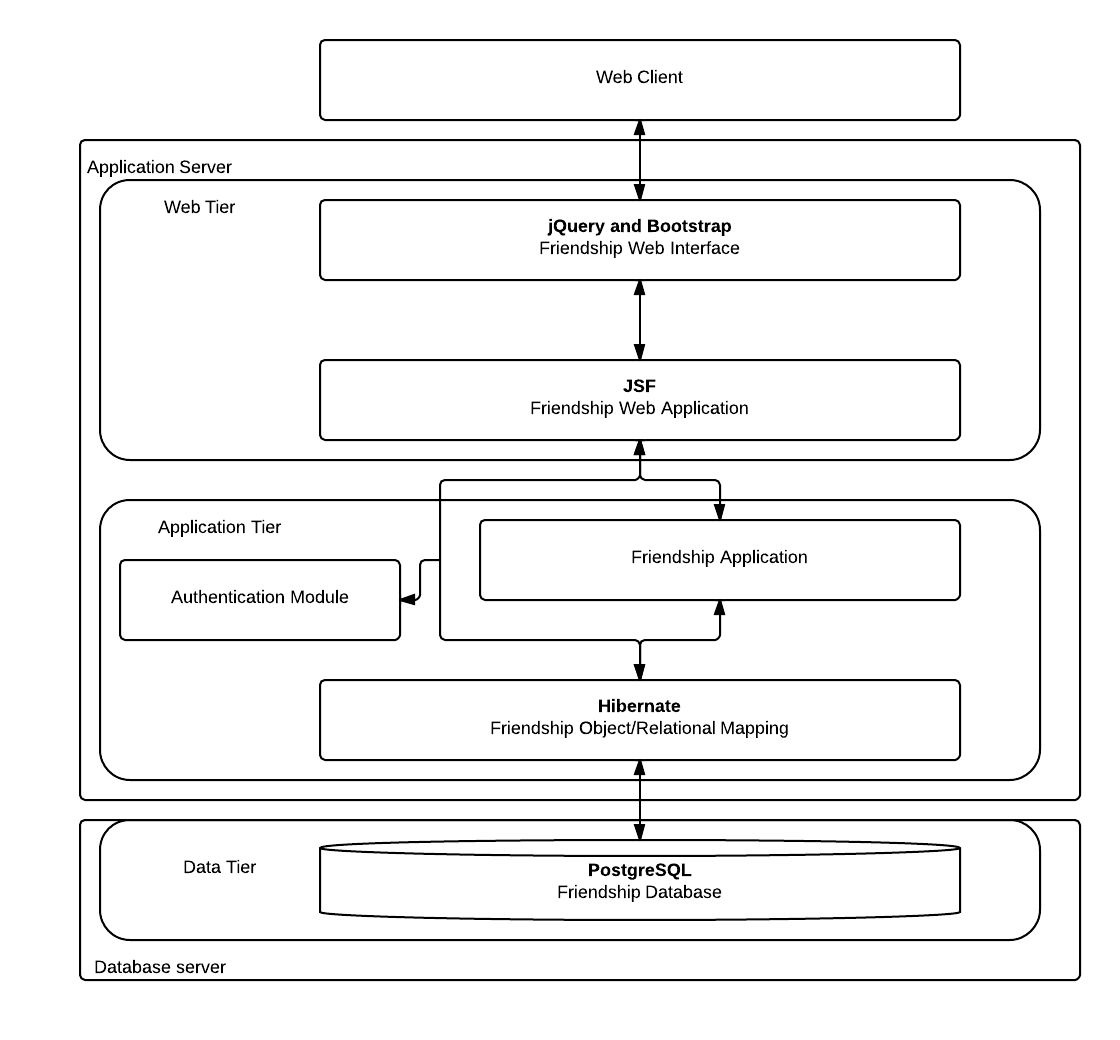
\includegraphics[scale=0.3]{ForestView}
\caption{Forest View diagram}
\label{fig:forest_view}
\end{figure}
\section{System Specification}

\subsection{Functional Requirements}
\begin{itemize}
\item A database model supporting users with the following data represented:
  \begin{itemize}
  \item User
      \begin{itemize}
      \item Usernamae
      \item Email
      \item Password
      \item Name
      \item Address
      \end{itemize}
  \item Hobbies
  \item Friends/romances
  \end{itemize}
\item CRUD for users
	\begin{itemize}
    \item Users should be able to view/edit their own data
    \item Admins should be able to create/delete users
    \item Users should be able to view others' data partially
    \end{itemize}
\item User authentication
\item Admin authorization
\item Browse or search functionality
\end{itemize}

\subsection{Non-functional requirements}
\begin{itemize}
\item The application is available through an HTTP connection 99.99\% of the time
\item A logging framework is enabled that allows the team to identify the underlying causes any breaches that may occur
\end{itemize}

\subsection{Security Requirements}
\begin{itemize}
\item A firewall blocks requests on all ports but port 80 (HTTP) and port 6666 (SSH)
\item Database access credentials are never stored in any source code repository
\item The database is always accessed in a manner that protects against SQL injection
\item The application guards against cross-site scripting
\end{itemize}

\section{System Design}
\subsection{Domain}
The domain is based on the user stories.


\begin{figure}[h!]
\centering
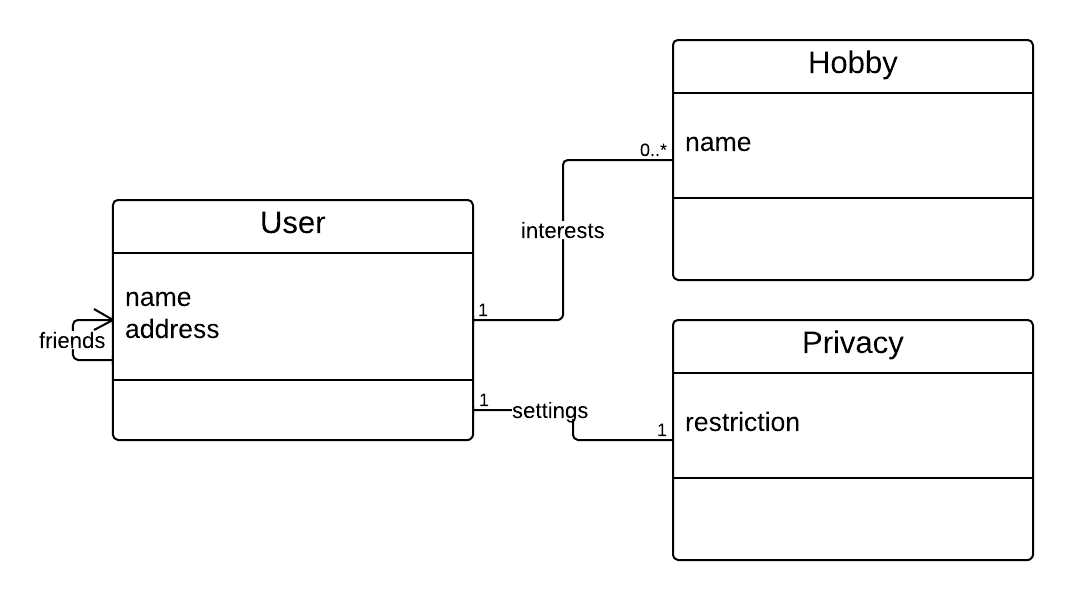
\includegraphics[scale=0.3]{Domain}
\caption{Domain diagram}
\label{fig:domain_diagram}
\end{figure}

\subsection{ER modelling}


\begin{figure}[h!]
\centering
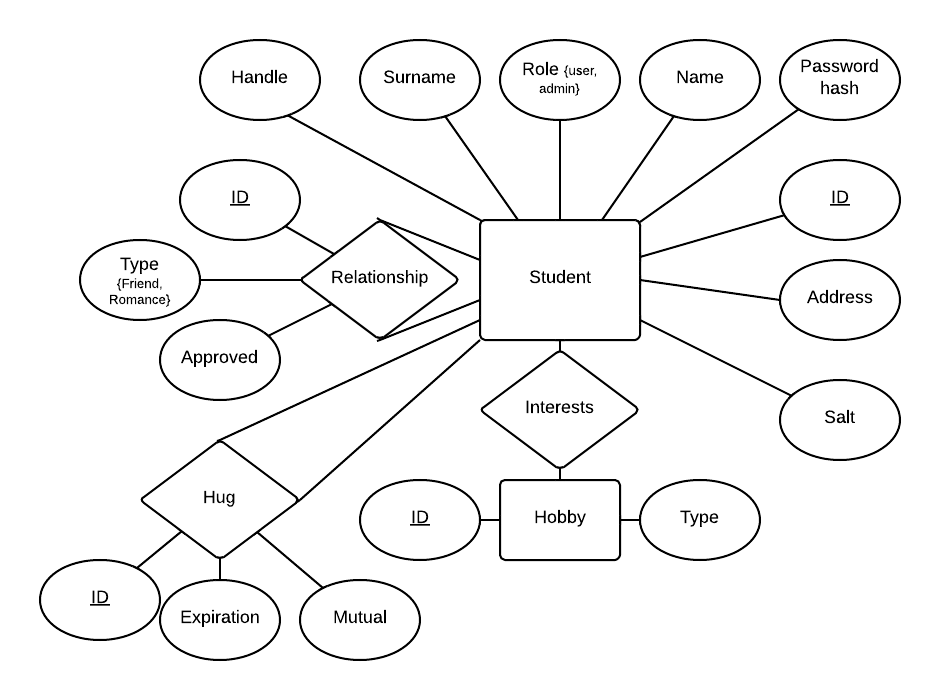
\includegraphics[scale=0.5]{ER}
\caption{Entity relationship diagram of our data-model}
\label{fig:er_diagram}
\end{figure}



\subsection{Choice of Technology}
\subsubsection{Frameworks and Technologies}
The following is a list of all the frameworks and technologies we have decided to use, with a short justification for each.
\begin{itemize}
\item \textbf{JSF2} is the recommended dynamic web page technology for this course, which makes help more readily available. In addition, we are all fairly experienced with Java, and one person on the team has prior experience with JSF. It provides protection against XSS and CSRF. \textbf{(TODO: Ensure that we actually do use JSF2 and not 1.21)}
\item \textbf{Tomcat 7} is a web application server, as with the above, is the recommended server technology.
\item \textbf{UFW}, the Uncomplicated Firewall, is a straightforward firewall implementation for Linux.
\item \textbf{Hibernate} is a library that provides ORM and can encapsulate database access in transactions and maps objects to relations.
\item \textbf{PostgreSQL} is our chosen database technology. Among other things, it provides fine-grained user access control.
\item \textbf{JUnit and Selenium with Selenide} for testing our application. JUnit provides a unit-testing framework for Java, which Selenium integrates with. Selenide is a framework for running tests for a web application through the browser.
\end{itemize}


\textbf{SHA-256} algorithm for hashing our users' passwords. It is generally regarded as a considerably secure hashing algorithm.
We also use a randomly generated 4 character salt for every user.

\subsubsection{Project Tools}
We have chosen to use the following tools to assist us in our project process.
\begin{itemize}
\item \textbf{Git} is our chosen tool for source control, since it is easy to use and gets the job done, and Github is a decent platform for hosting source code on.
\item \textbf{Google Docs} is what we use for taking notes and making on-the-fly documents, spreadsheets or presentations that we might need throughout the project. It is very easy to share things here, but the text processing tool is not that powerful, so it is not where we write our report.
\item \textbf{writeLaTeX} is a web application that offers collaboration on LaTeX documents. This is the tool we use for writing the report, since LaTeX is a powerful text processing tool and writeLaTeX gives us the collaborative functionality.
\end{itemize}

\subsection{Architecture}

\subsubsection{Principles}

Our production server runs Linux and provides the access control for users' access to the file system.

We have attempted to restrict privilege given on our server so users are given 
\textbf{Least Privilege} as possible to the file system. We have disabled remote login for the root user and every member of the team has a user that is in a superuser group. The application server and database runs each with their respective user that is only used for that process. However we need to give root access to the application server because it needs to run on port 80.


Our database is our most valuable asset and therefore we wish to protect it. The database user/role for the database creation is different from the user that is used by the application server. By applying this practice we give the application the least possible privilege to the database to protect our database from being dropped. Furthermore we store the username and password to the database on the server and we don't share the username and password in our VCS according to the principle of \textbf{Reluctance to Trust} since we don't trust the confidentiality of our VCS.

Our application authorizes users in order to determine the privilege for access to user stories like pages that a user has.

We replaced the error page in order to \textbf{Fail Securely}.


\section{Testing}
\subsection{Tools and Frameworks}
Testing is essential in order to build secure and functional software systems. To thoroughly test our system we have decided to use two testing strategies; system tests and unit tests.

A testing tool we found fitting to use for system tests is Selenium with JUnit. Selenium allows us to script test cases which input data and submit forms on the webservice.

\subsection{System test cases (Black-box Test)}

\begin{itemize}
\item Login
\item SQL injection in input
\item Access to unauthorized pages
\item Creating user
\item Renewing password
\end{itemize}


\section{Hacking}
\subsection{Plans and ideas}
In this section we describe plans and ideas for hacks and attacks that we haven't (yet) conducted.
\subsubsection{Social engineering attack}
A social engineering attack requires some knowledge and analysis of the setting, system and people you want to attack.

The setting at hand is that we are among a set of teams all implementing and trying to secure a webservice which must be "handed in" and shown off to a teacher and possibly the TA. This implies that the people in the teams all trust both the teacher and the TA. We have observed that most of us do not remember the name of the TA off the top of our heads and need to look it up on the course blog.
We can use this knowledge to make a broad social engineering attack on all other groups attempting to obtain confidential information such as usernames and passwords for admin accounts.

The idea is to send an email to the entire class that looks and sounds official and says that it is from ``The TA of System Architecture and Security F2013". We assume that the students are not aware of the name of our TA and that they will trust that if we claim to be him in the email, they will believe us. The email will contain a request for login information to their webservice for an admin account that we need in order to evaluate the teams' progress.

A requirement for this attack to work is that we send the email before (if) the teacher or TA asks for this information from the groups. We plan on sending the email on the 4th of October.


\textbf{Team 1}

%Inserted the following as username and password in login form:
%\begin{verbatim}
%' OR 1 = 1;--
%\end{verbatim}
%This resulted in a 502 error followed by errorcode 500 responses on following %attempts at reaching the website.
%In order to submit the form the in-browser email verification had to be disabled %(achieved by editing the DOM such that type="email" became type="text")


\section{Discussion}
\subsection{Problems}
\subsection{Deployment}

\subsection{...}


\section{Conclusion}

\section{Appendix}
\textbf{Team contract}

The team consists of the following four members:
\begin{itemize}
\item{Jacob Fisher (jaco@itu.dk)}
\item{Christian Lyngbye (clyn@itu.dk)}
\item{Ivaylo Sharkov (isha@itu.dk)}
\item{Rasmus Greve (ragr@itu.dk)}
\end{itemize}
Our expectations of the project is to create a working product with a report meeting all requirements at the right deadlines. We expect to get at least a passing grade and strive towards getting a 10 or 12 at the exam.

We agree on doing project work at least once a week, usually on fridays from 10am to around 2-4pm depending on the amount of work to be done and the deadlines.

Three group members have an exam in week 42. After this, we should be able to meet some Thursdays as well.

Rasmus is having a baby in the end of October and will not be able to do group work on site at ITU in a couple of weeks after this time. He will do work from home and keep in touch with the group via email and instant messaging.

\textbf{Week 37 (13/09/2013)}

Today we created our course log and a git repository.
Jacob retrieved information for our server slice.

We decided on which technologies we were going to use:
We would use the programming language Java and create a Web Application that would use JSF and ORM to map objects to a relational database.

We chose to user a Tomcat server as the application server.

For source control management we have shared a private repository on Github.

We made some agreements in the group regarding collaborative tools.
We chose to use LaTeX to write the report and hosted it on writeLaTeX.
Google Drive for file sharing.
Facebook for communicating outside of the university.

On the server slice we set up a firewall to filter all ports except 6666 which we use for SSH.
We disallowed root access to SSH.
In order to run the application on the server we downloaded and installed: Java JDK, Apache Tomcat and Git.
We discussed how to deploy to the server and considered building the application locally on the server.

We made an initial draft of user stories and requirements for our system.


\textbf{Week 38 (20/09/2013)}

As an experiment Christian installed PostgreSQL on the server slice and it was proved to work so we chose to use it. 
Christian scanned all team servers with nmap and found some differences in solutions e.g. turning ping responses off and closed ports.
Added an example Netbeans project with JSF and started working on connecting to the database.
Rasmus designed the database diagram created an initial creation script for the database.

Ivaylo analyzed the risks.

Planned to do code review and architectural risk analysis.


\textbf{Week 39 (27/09/2013)}

This week we began work on the project report by determining which chapters we need. Jacob started writing the choices of technology chapter and the introductory chapters.

The goal and risk analysis was elaborated on and importet into the report LaTeX document.

We discussed and planned a social engineering attack targeted at all the other groups involving impersonating the TA in an email. We agreed that it was still too early in the process to perform this attack since most teams would be unlikely to have a working webservice to which we could gain access.

\textbf{Week 40 (04/10/2013)}

Ivaylo was sick today and was unable to do group work.

Christian made some refactoring in the codebase requiring the rest of the team to reimport the project into NetBeans.
This refactoring included renaming the project and introducing the Selenide testing framework and a few sample test cases to be elaborated on later. The system is now called ``FriendSpace''.

Rasmus spent a bit of time styling the webpages using Twitter Bootstrap. Jacob drew a logo to make the visual expression of the webpages more appealing.

The system was deployed to the webserver on port 80 which was opened. Accessing the root of the server redirects the user to /ssase13.

Furthermore, the team spent a lot of time throughout the day finishing up the first draft of the report for the first hand-in.


\textbf{Week 41 (11/10/2013)}


\textbf{Week 42 (18/10/2013)}


\textbf{Week 43 (25/10/2013)}

Worked on Sins presentation about Race Conditions. This led to some improvements of our code.

\textbf{Week 44 (01/11/2013)}
\textbf{Week 45 (08/11/2013)}

Reorganized the report into distinct sections.
Divided work between us to help organize.

\textbf{Week 46 (15/11/2013)}

Implemented friend requests.
Rewrote risk analysis to use the book structure.

\end{document}